\section{Thermoelastic plate (2D)}
\label{sec:tm2d}
\subsection{Definition}
We consider a thermoelastic consolidation on a 2D vertical plate under plane strain conditions. All parameters are dimensionless. The domain has a rectangular shape with size of 10 $\times$ 10. Material properties are listed in Table \ref{tab:tm2D}. Initial condition is given by
\[
\mathbf \sigma_{0} = \mathbf 0, \, T_0=198.15
\]
and boundary conditions are depicted in Figure \ref{fig:TMbc}. Gravity force is considered in $y$ direction. 

\begin{table}[!htb]
\caption{Model parameters}
\label{tab:tm2D}
\centering
\begin{tabular}{llrr}
\toprule
Symbol & Parameter & Value & Unit \\
\midrule
$E$ & Young's modulus & $3 \cdot 10^{3}$  & $-$ \\
$\nu$ & Poisson's ratio & $0.3$       & $-$ \\
$\rho$ & Density    & $1.0$        & $-$ \\
$\beta$ & Volumetric thermal expansion & $1.0$         & $-$ \\
$c$ & Specific heat capacity & $1.0$         & $-$ \\
$\lambda$ & Thermal conductivity & $1.0$         & $-$ \\
\bottomrule
\end{tabular}
\end{table}

\begin{figure}[!htbp]
\centering
%\input{PART_III/TM/e1.eepic}
\epsfig{figure=PART_III/TM/figures/e1,height=5cm}
\caption{Boundary conditions for TM coupling plane strain problem }
\label{fig:TMbc}
\end{figure}

\subsection{Solution}
%\subsubsection{Analytical solution}
%\subsubsection{Numerical solution}
%%The results are compared with the analytic solution as well.
%All parameters are dimensionless. 
Numerical simulation is conducted with time step size 0.1. The simulation runs 100 steps. The domain is discretized into quadrilateral elements (Figure \ref{fig:TM2Mesh}). 

%\begin{figure}[!htb]
\begin{figure}[!htbp]
\centering
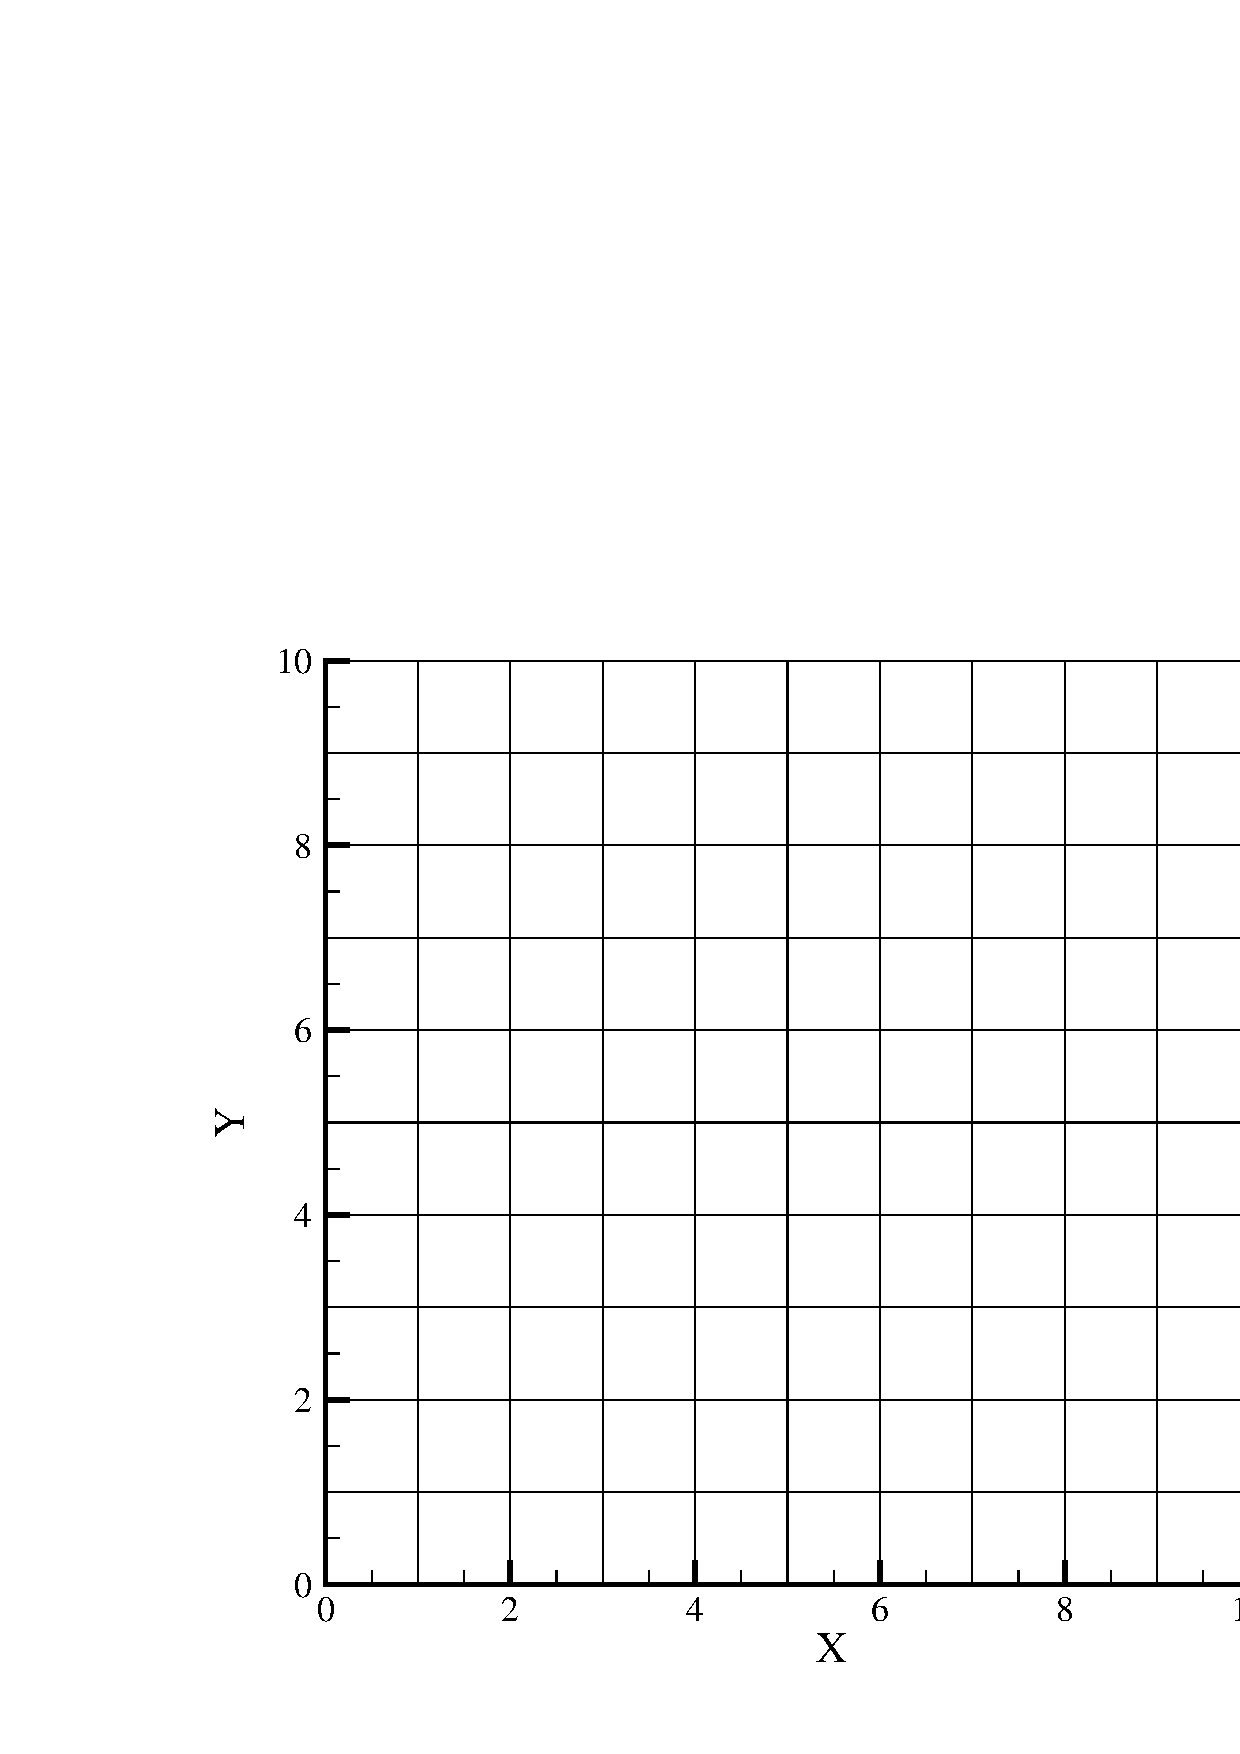
\includegraphics[height=5cm]{PART_III/TM/figures/2D_mesh}\\
\caption{Mesh for TM coupling plane strain problem }
\label{fig:TM2Mesh}
\end{figure}




\subsection{Results}
Fig. \ref{fig_TM1_r} provides the distribution of temperature and vertical stress after 100 time steps. The vertical stress distribution shows the effect of gravity force. The results of 2D model are compared with that of 3D model in the next example.

%\begin{figure}[!htb]
\begin{figure}[!htbp]
\begin{center}
\epsfig{figure=PART_III/TM/figures/2D_T,height=6cm}
\epsfig{figure=PART_III/TM/figures/2D_syy,height=6cm}
\end{center}
\caption{Distribution of temperature and vertical stress after 100 time steps}
\label{fig_TM1_r}
\end{figure}

